\documentclass[a4paper,12pt]{article} 
% Paquetes......................................................................
\usepackage{amsmath, amssymb, amsfonts, latexsym}
\usepackage[utf8]{inputenc}
\usepackage[T1]{fontenc}
\usepackage{palatino}
\usepackage[full]{textcomp}
\usepackage{hyperref}
\usepackage{eurosym}
\usepackage[makeroom]{cancel}
\usepackage{array}
\usepackage{pdfpages}
\usepackage{float} % para que las figuras no floten
\usepackage{subcaption}
\usepackage{soul}
\usepackage{pythonhighlight} % para el entorno python de listings

\textheight = 24 cm
\textwidth = 17 cm

\renewcommand{\arraystretch}{1.25}
\renewcommand{\contentsname}{Contenidos}


% INICIO DEL DOCUMENTO --------------------------------------------------------
\begin{document}
	
	\setlength{\parindent}{0.5cm}
	\setlength{\voffset}{-2cm}
	\setlength{\hoffset}{-2cm}
	
	
	%%%%%%%%%%%%%%%%%%%%%%%%%%%%%%%%%%%%%%%%%
% Academic Title Page
% LaTeX Template
% Version 2.0 (17/7/17)
%
% This template was downloaded from:
% http://www.LaTeXTemplates.com
%
% Original author:
% WikiBooks (LaTeX - Title Creation) with modifications by:
% Vel (vel@latextemplates.com)
%
% License:
% CC BY-NC-SA 3.0 (http://creativecommons.org/licenses/by-nc-sa/3.0/)
% 
% Instructions for using this template:
% This title page is capable of being compiled as is. This is not useful for 
% including it in another document. To do this, you have two options: 
%
% 1) Copy/paste everything between \begin{document} and \end{document} 
% starting at \begin{titlepage} and paste this into another LaTeX file where you 
% want your title page.
% OR
% 2) Remove everything outside the \begin{titlepage} and \end{titlepage}, rename
% this file and move it to the same directory as the LaTeX file you wish to add it to. 
% Then add \input{./<new filename>.tex} to your LaTeX file where you want your
% title page.
%
%%%%%%%%%%%%%%%%%%%%%%%%%%%%%%%%%%%%%%%%%

%----------------------------------------------------------------------------------------
%	PACKAGES AND OTHER DOCUMENT CONFIGURATIONS
%----------------------------------------------------------------------------------------


%----------------------------------------------------------------------------------------
%	TITLE PAGE
%----------------------------------------------------------------------------------------

\begin{titlepage} % Suppresses displaying the page number on the title page and the subsequent page counts as page 1
	\newcommand{\HRule}{\rule{\linewidth}{0.5mm}} % Defines a new command for horizontal lines, change thickness here
	
	\center % Centre everything on the page
	
	%------------------------------------------------
	%	Headings
	%-----------------------------------------s-------
	
	\textsc{\Large Máster en Inteligencia Artificial}\\[1.5cm] % Main heading such as the name of your university/college
	
	\textsc{\LARGE Métodos de simulación}\\[0.5cm] % Major heading such as course name
	
	%\textsc{\large Minor Heading}\\[0.5cm] % Minor heading such as course title
	
	%------------------------------------------------
	%	Title
	%------------------------------------------------
	
	\HRule\\[0.4cm]
	
	{\huge\bfseries Práctica Grupo 3}\\[0.4cm] % Title of your document
	
	\HRule\\[1.2cm]
	
	%------------------------------------------------
	%	Author(s)
	%------------------------------------------------
	
	%\begin{minipage}{0.4\textwidth}
	%	\begin{flushleft}
	%		\large
	%		\textit{Author}\\
	%		\textsc{Aída Muñoz Monjas} % Your name
	%	\end{flushleft}
	%\end{minipage}
	%~
	%\begin{minipage}{0.4\textwidth}
	%	\begin{flushright}
	%		\large
	%		\textit{Supervisor}\\
	%		Dr. Caroline \textsc{Becker} % Supervisor's name
	%	\end{flushright}
	%\end{minipage}
	
	% If you don't want a supervisor, uncomment the two lines below and comment the code above
	{\Large\textit{Autores}}\\
	
	{\large\textsc{Luis Couto seller\\
			 Irene Marbán Álvarez\\
			 Aída Muñoz Monjas} } % Your name
	
	%------------------------------------------------
	%	Date
	%------------------------------------------------
	
	\vfill\vfill\vfill % Position the date 3/4 down the remaining page
	
	{\large\today} % Date, change the \today to a set date if you want to be precise
	
	%------------------------------------------------
	%	Logo
	%------------------------------------------------
	
	%\vfill\vfill
	%\includegraphics[width=0.2\textwidth]{placeholder.jpg}\\[1cm] % Include a department/university logo - this will require the graphicx package
	 
	%----------------------------------------------------------------------------------------
	
	\vfill % Push the date up 1/4 of the remaining page
	
\end{titlepage}

%----------------------------------------------------------------------------------------

%\end{document}

	
	\tableofcontents
	
\newpage
	\section{Generación de números y variables aleatorias}
	
	\subsection{Enunciado}
	
	Describir el método \textit{Monty Phyton} para la distribución normal y compararlo con otros métodos para la generación de valores de la normal.
	
	\subsection{El método Monty Python}
	
	El objetivo del método Monty Python es lograr generar números aleatorios cuya frecuencia se aproxime a aquella de una distribución normal. Para ello, emplea la similitud entre la expresión de la función de densidad de la distribución normal y una sigmoide decreciente, así como se aprovecha del bajo coste computacional de la generación de números aleatorios en un rectángulo.
	$$ N(0,1) \sim f(x) = \dfrac{1}{\sqrt{2\pi}} \cdot e^{-x^2/2} $$
	
	Tomando $x>0$, se traza un rectángulo de base $b$ y altura $1/b$ sobre la sigmoide. Con un giro de $\pi$ radianes y un desplazamiento sobre la región exterior al rectángulo se pretende representar la mayor superficie posible de la sigmoide en el interior del rectángulo de área $1$. En las imágenes siguientes, podemos observar el procedimiento descrito tomando un $b=2.29$.
	\vspace{-1mm}
	\begin{figure}[H]
		\begin{subfigure}{.5\textwidth}
			\centering
			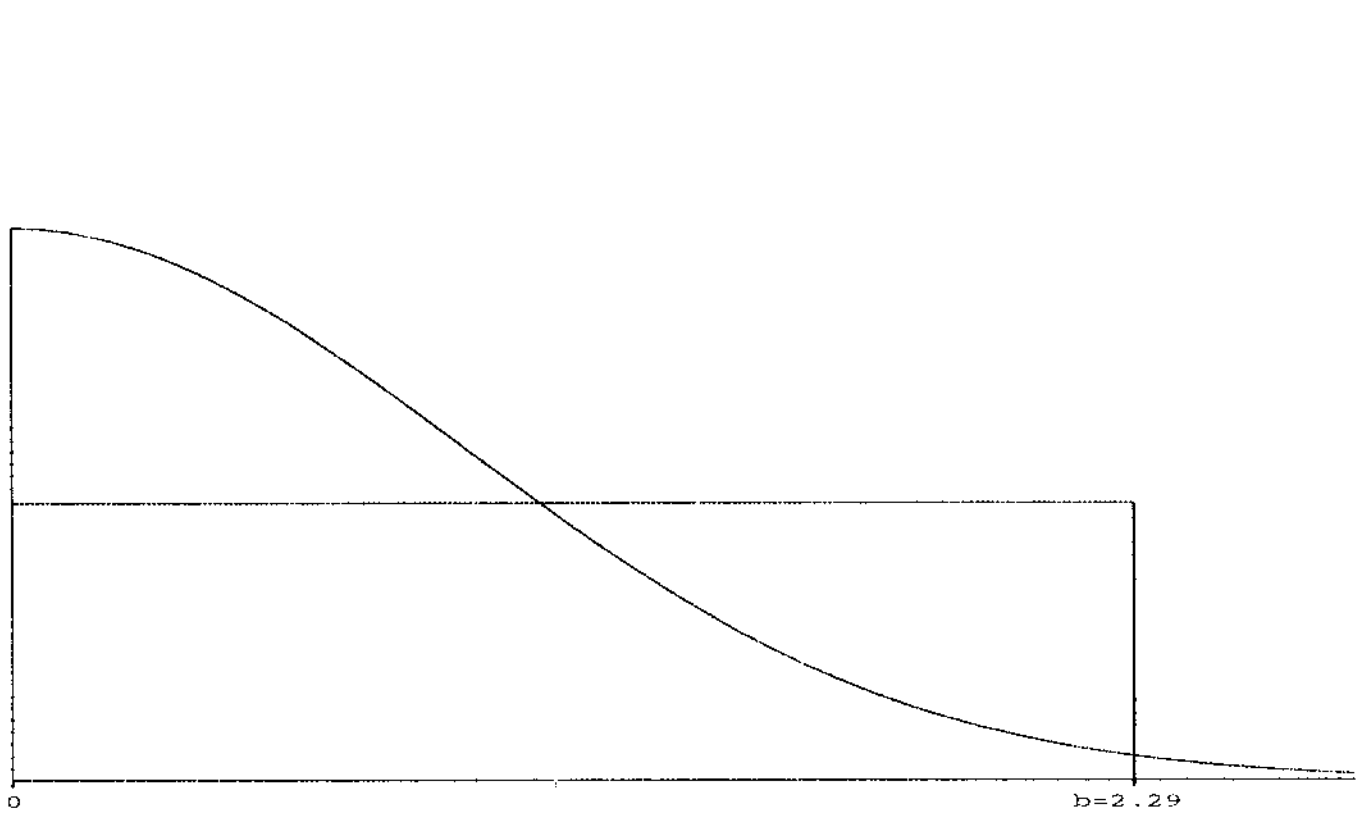
\includegraphics[width=\textwidth]{include/sigmoid_w_square.png}
			\caption{Sigmoide con el rectángulo de base $b$. \cite{monty-python}}
		\end{subfigure}
		\begin{subfigure}{.5\textwidth}
			\centering
			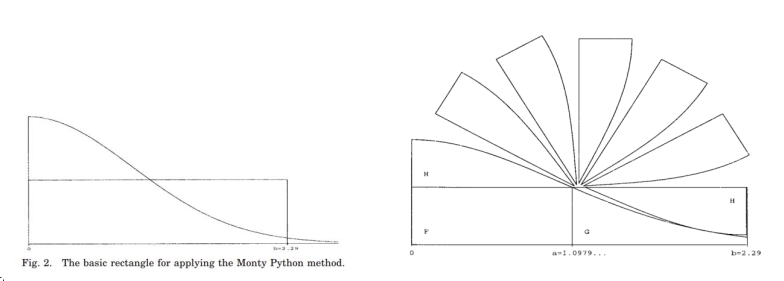
\includegraphics[width=\textwidth]{include/rotating_sigmoid.png}
			\caption{Giro y desplazamiento gráficamente. \cite{monty-python}}
		\end{subfigure}
	\end{figure}
	
	Una vez descrito el área bajo la función de densidad en el interior del rectángulo, todo número aleatorio generado en ese rectángulo pertenecerá a las regiones $F$, $G$, $H$ o a la región comprendida entre $G$ y $H$ correspondiente a la cola de la sigmoide. La probabilidad de obtener un número en la cola es de un $0.022$ \cite{monty-python}.
	
	Siendo $(x,y)$ el valor aleatorio generado, $(x',y')$ será su valor correspondiente en la sigmoide.
	$$
	(x',y') = 
	\begin{cases}
		(x,y) \quad \text{si} \quad x\in F \text{ ó } G \\
		(b-x,2/b-y) \quad \text{si} \quad x \in H
	\end{cases}
	$$  
	
	Si el valor aleatorio generado no pertenece a $F$, $G$ ó $H$, pertenecerá a la cola de la distribución, por lo que basta con devolver una variante de la cola normal mediante el método de Marsaglia o el método de la cola general de Marsaglia y Tsang.\\
		
	La elección del valor de $b$ no es crítica, pero elegir un valor de $b$ demasiado grande implica que habrá solapamiento al realizar el giro y desplazamiento descrito, mientras que si el valor de $b$ es demasiado pequeño, será necesario realizar frecuentemente el método para hallar los valores de la cola.
	En caso de utilizar el método anterior para "ajustar" la sigmoide al rectángulo, la elección de $b=2.29$ es prácticamente la máxima posible \cite{monty-python}. \\
		
	En lugar de una rotación y un desplazamiento de la región exterior al rectángulo, "estirar" la región $H$ permite un ajuste mejor, manteniendo constante el área de la sigmoide, y por tanto siendo este un método más complejo pero más eficiente para realizar dicha aproximación. 
	
	Definiendo el factor de estiramiento $s$ y la función de densidad de la región $H$, $f_H(x)$, 
	$$s=\dfrac{a}{b-a} \hspace{1.5cm} f_H(x)=f(x)-\dfrac{1}{b} \hspace{2mm} \text{con} \hspace{2mm} 0<x<a $$
	se tiene que la región $H$ girada y estirada tiene una función de densidad $f_{H'}(x)$.
	$$ f_{H'}(x) = \dfrac{1}{b} - s  \left[ f(s (b-x) ) -\dfrac{1}{b} \right] $$ 
	La siguiente figura representa gráficamente las transformaciones matemáticas descritas compuestas con la rotación aplicada a la sección $H$. 
	
	\begin{figure}[H]
		\centering
		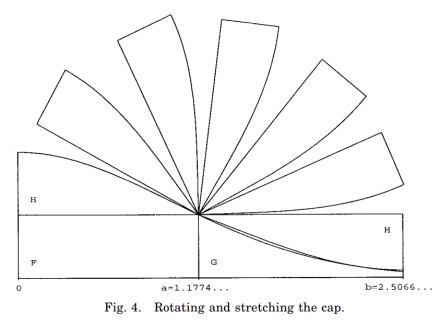
\includegraphics[width=0.6\textwidth]{include/stretching_sigmoid.png}
		\caption{Descripción gráfica del estiramiento descrito. \cite{monty-python}}
	\end{figure}
	
	Para este segundo caso, la elección habitual para el valor de $b$ es $b= \sqrt{2\pi}$. Esta elección no es crítica, cualquier valor entre $2.506$ y $2.5074$ es válido \cite{monty-python}, pero el par $b=\sqrt{2\pi}$, $a = \sqrt{\ln 4}$ son opciones fácilmente identificables con una precisión ilimitada.
	
	
\newpage
	\subsection{Comparación de métodos}
	A continuación, se compararán diferentes métodos para la generación de valores de la normal con el método Monty Python. Para ello, nos basaremos en la publicación citada \cite{comparacion-metodos}. Teniendo en cuenta que tanto el método generador de las secciones $F$, $G$ y $H$, como el método generador de las colas de la sigmoide son relevantes, el artículo divide la evaluación en cuatro secciones.

	
	\begin{itemize}

		\item Tests de bondad de ajuste. Para evaluar los algoritmos utilizados, se utiliza el test $\chi^{2}$. El número de intervalos en los que se divide la distribución para realizar el test es $k$, que se define mediante la siguiente expresión, siendo $n$ el número de muestras.

		\vspace{-5mm}
		$$k = \lceil n^{3/5} \rceil $$
		
		\item Test para valores altos de sigma. Este test mide principalmente el comportamiento de los generadores en las colas de la distribución. El principal reto es la baja probabilidad de obtener muestras que se encuentren en las colas. Se utiliza por tanto un algoritmo para "forzar" la generación de muestras que sean grandes múltiplos de sigma. 

		
		\item Test de aleatoriedad. Para este test, se utiliza la batería Crush, que forma parte de los \textit{TestU01}.

		
		\item Test de correlación interbloque. Este test mide como afecta la distribución de cada una de las muestras a la muestra siguiente, considerándose un buen resultado si la distribución de cada una de las muestras es independiente de las anteriores.

	\end{itemize}

	
	También se evalúa el número de operaciones realizadas y la velocidad de ejecución. 
	
	\subsubsection{Resultados en velocidad.}
	La velocidad se mide relativa a la velocidad del método de Rechazo Polar. El método Monty Python es el cuarto más rápido en comparación con los $16$ otros métodos de generación de variables aleatorias estudiados \cite{comparacion-metodos}, siendo $1.61$ veces más rápido que el método de Rechazo Polar. Cabe destacar que el número de operaciones realizadas es bajo en comparación con el método Wallace, que está por encima del método Monty Python en rapidez. Este último tiene menos cantidad de constantes que el método Ziggurat, que está también por encima del Monty Python en cuestión de velocidad.
	
	\begin{table}[H]
		\centering
		\begin{tabular}{|c||c|}
			\hline
			Nombre del método     & Velocidad     \\ \hline \hline
			Wallace (qual=1)      & 6.41          \\ \hline
			Ziggurat              & 4.29          \\ \hline
			Wallace (qual=4)      & 2.48          \\ \hline
			\textbf{Monty Python} & \textbf{1.61} \\ \hline
			PPND7                 & 1.16          \\ \hline
			Mixture-of-triangles  & 1.14          \\ \hline
			Polar                 & 1.00          \\ \hline   
		\end{tabular}
	\end{table}
	
	\subsubsection{Resultados en el test de bondad de ajuste $\chi^{2}$.}
	En el test de bondad de ajuste $\chi^{2}$, el método Monty Python no pasa el test al utilizar muestras de valores mayores a $2^{34}$. De nuevo, los métodos Wallace y Ziggurat obtienen mejores resultados, ya que no fallan al utilizar muestras de valor igual o mayor a $2^{36}$. El algoritmo PPND7 falla en la misma prueba que el método Monty Python, que a su vez es $3$ veces más lento.
	
	\subsubsection{Resultados en el test de valores altos de sigma.}
	Los resultados de este test muestran el múltiplo más alto de sigma donde el test se realiza con éxito. El método Monty Python obtiene un valor de $8.27$, siendo en este caso mejor que los métodos Ziggurat y Wallace. En comparación con el resto de generadores, el método Monty Python obtiene muy buenos resultados, situándose el cuarto mejor de todos los generadores comparados.
	
	\subsubsection{Resultados del test de aleatoriedad}

	El generador Monty Python no tuvo fallos al realizarse el test Crush.
	
	\subsubsection{Resultados del test de correlación interbloque.}
	Este test solo se realizó en los generadores Ziggurat, Wallace y Monty Pythhon, dado que fueron los más rápidos y en este test se necesitan realizar pruebas con muestras muy grandes. Los generadores de Ziggurat y Monty Python pasaron todos los tests con éxito, mientras que el generador Wallace (tanto el de baja calidad como el de alta), falló con un número inferior a $8$ iteraciones. Esto se debe a que el método Wallace es recursivo.
	
	\subsubsection{Conclusiones}
	Si bien es cierto que el método Wallace es el más rápido, presenta desventajas evidentes como la correlación. 
	El método Ziggurat, que es más lento que el Wallace, no tiene problemas de correlación, pero si que falla en el test Crush con una colisión identificada en los tests de doble precisión. 
	Además, utiliza un total de $388$ constantes, lo que puede ser problemático en algunos entornos. 
	El método Monty Python es el tercero más rápido después del Wallace y el Ziggurat, y presenta ventajas evidentes, como los buenos resultados en los tests de aleatoriedad y correlación, así como el bajo número de operaciones y constantes necesarias. 
	La mayor limitación del método Monty Python está en el uso de muestras cuya $n$ sea mayor que $2^{36}$. 
	
	
	\newpage

	\section{Simulación de sucesos discretos y optimización}

	\subsection{Enunciado}
	Consideremos un almacén de dos productos cuyos precios de venta al público son de $2.5$ y $3.5$ euros la unidad, respectivamente. La llegada de clientes al almacén se distribuye según un proceso de Poisson de parámetro $\lambda = 1.5$ clientes por hora y la cantidad de productos demandados por cada uno de ellos tiene la siguiente distribución:

	\begin{table}[H]
		\centering
		\begin{tabular}{|l||c|c|c|c|}
			\hline
			Demanda    & 1 unidad & 2 unidades & 3 unidades & 4 unidades \\ \hline \hline
			Producto 1 & 0.3      & 0.4        & 0.2        & 0.1        \\ \hline
			Producto 2 & 0.2      & 0.2        & 0.4        & 0.2        \\ \hline
		\end{tabular}
	\end{table}
	
	Para satisfacer la demanda de sus clientes el dueño del almacén mantiene un stock de productos. La política de pedidos al distribuidor es periódica, es decir todos los viernes a primera hora realiza un pedido, tomando como referencia el nivel de inventario de los productos en ese. Para satisfacer la demanda de sus clientes el dueño del almacén mantiene un stock de productos. La política de pedidos al distribuidor es periódica, es decir todos los viernes a primera hora realiza un pedido en el que tomando como referencia el nivel de inventario de los productos en ese momento, se solicitan las unidades necesarias para que el nivel del inventario de cada producto llegue a $1000$ y $1500$ unidades, respectivamente en cada producto.

	Asociado a cada pedido que realizamos al proveedor existe un coste fijo (coste de preparación) de $100$ euros, independientemente de las unidades demandadas. Adicionalmente, el coste por unidad incluida en el pedido depende de la cantidad solicitada habiendo descuentos por cantidad. Si el número de unidades demandadas del primer producto es menor o igual a $600$ el precio es de $1$ euro la unidad, mientras que si se piden más de $600$ el precio desciende a $75$ céntimos. Para el segundo producto, si el número de unidades demandadas es menor que $800$ el precio es de $1.5$ euros la unidad, mientras que si se piden más de $800$ el precio desciende a $1.25$ euros.

	El tiempo que tarda en ser servido el pedido por los proveedores (tiempo líder), sigue una distribución normal de media 48 horas y desviación típica $3.5$, pagándose en ese momento.

	Se ha llegado a un acuerdo con el proveedor de forma que, tomando como referencia las $48$ horas que tarda en media un pedido en ser servido, si el pedido llega con $3$ horas de retraso en la entrega del mismo se realiza un descuento del $0.03\%$ del valor del pedido, encareciéndose en la misma cantidad en el caso de que el pedido llegue con al menos $3$ horas de adelanto.
	
	El dueño del almacén debe pagar $0.0002$ euros por unidad del producto y unidad de tiempo, asociado al almacenamiento físico de los productos (alquiler del local, refrigeración...). En el caso de que al llegar un cliente éste solicite una cantidad mayor que la que hay en inventario, se le sirve lo que queda, perdiendo la venta restante.
	
	\begin{enumerate}
		\item[a)] Simular el comportamiento de almacén durante un periodo de tiempo de $5$ meses para estimar el beneficio esperado, la proporción de clientes cuya demanda se satisface completamente y el porcentaje de tiempo que el nivel del inventario permanece a cero. Para ello, supondremos que el nivel del inventario inicial es de $70$ unidades de ambos productos.

		\item[b)] Representar gráficamente la evolución del nivel del inventario durante los $5$ meses y durante los $5$ primeros días. 

		\item[c)] Mediante el uso de la metaheurística recocido simulado identificar cuál será la política de pedidos óptima, es decir, identificar cada cuánto tiempo se deberían realizar los pedidos y el valor de referencia del inventario para identificar el número de unidades a solicitar en la política de pedidos periódica.
	\end{enumerate}
	
	\textbf{Nota.} El almacén permanece abierto las $24$ horas al día de lunes a domingo. El proveedor y la empresa transportista (que sirve los pedidos) también trabajan las $24$ horas, no cerrando en ningún momento.

	\subsection{Modelado del problema}
	El problema descrito se puede representar según el diagrama a continuación.
	
	\begin{figure}[H]
		\centering
		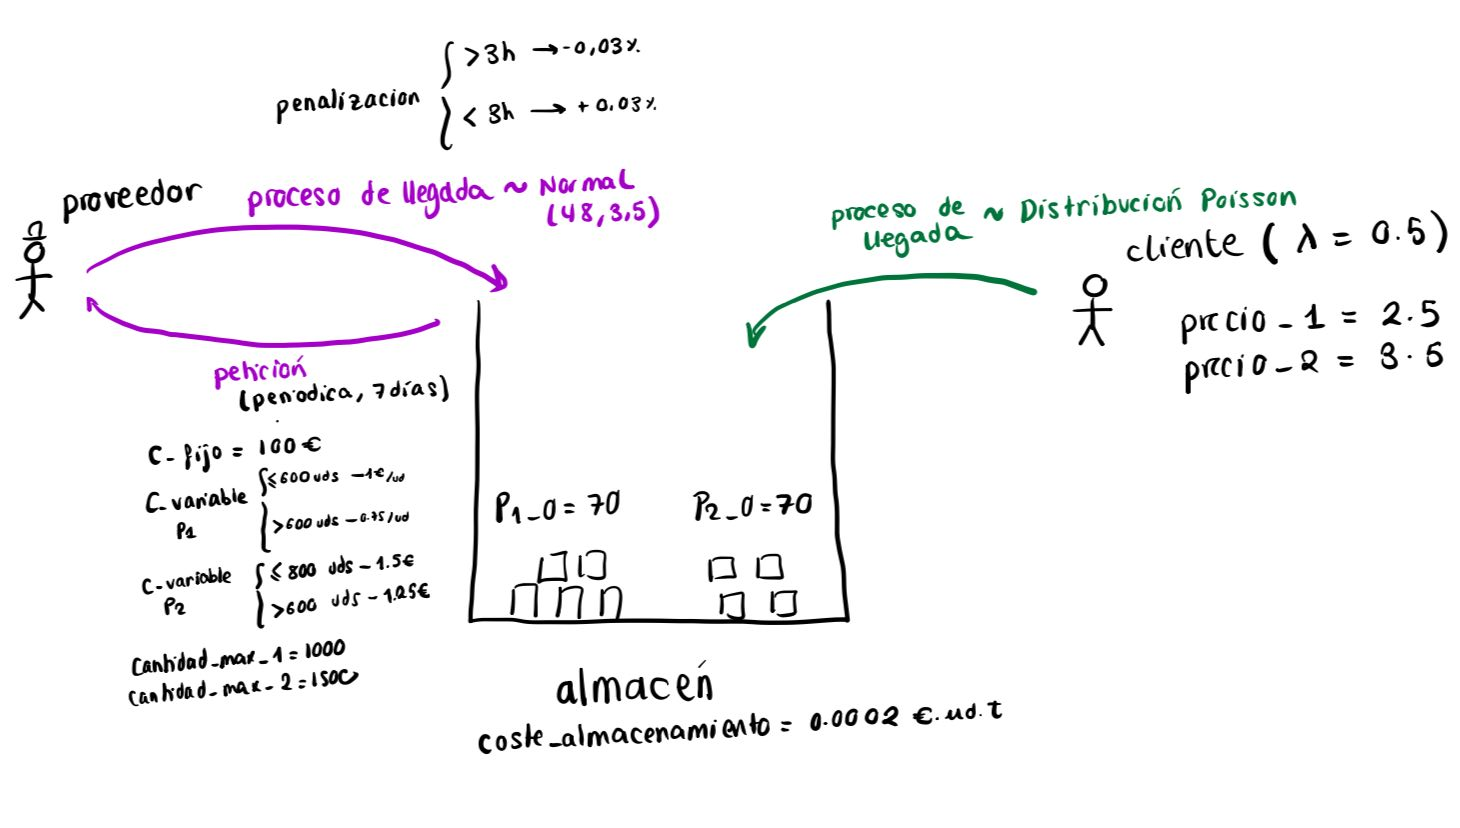
\includegraphics[width=\textwidth]{include/modelo_almacen.png}
		\caption{Representación gráfica del modelado del problema}
	\end{figure}
	
	El almacén guarda productos de dos tipos, siendo $x_1$ y $x_2$ la cantidad de cada uno de los productos almacenados en un instante. Los productos se guardan por separado, teniendo una cantidad máxima de cada producto en stock.
	
	Una de las principales características de este problema es su política de pedidos. Cada $7$ días el propietario realiza un pedido al proveedor, independientemente del estado del almacén durante los días anteriores.
	
	La llegada de clientes al sistema sigue una distribución de Poission con $\lambda = 0.5$, mientras que la llegada de pedidos sigue una normal $N(48, 3.5)$.
	
	El coste total del sistema se calcula como las ganancias por las ventas de productos ($R$) menos los costes de almacenamiento ($H$) y costes de compra de productos al proveedor ($C$).
	
	
	
	\subsection{Simulación del problema. Estimación de beneficios y satisfacción de clientes.}
	Según lo indicado en el apartado a), el objetivo de esta sección es obtener los siguientes valores.
	\begin{itemize}
		\item Estimación el beneficio esperado.
		\item Proporción de clientes cuya demanda se satisface completamente.
		\item Porcentaje de tiempo que el nivel del inventario permanece a cero.
	\end{itemize}
	Se simulará el comportamiento del sistema durante $5$ meses, teniendo inicialmente $70$ unidades de ambos productos en el almacén.
	 	
	\subsubsection{Implementación}
	La implementación de esta simulación se realizó utilizando el lenguaje python, definiendo de manera separada las rutinas de llegada de un cliente, llegada de un pedido y compra de un pedido.
	
	Las variables utilizadas se definen como globales, permitiendo que la entrada de cada uno de los métodos sea únicamente el tiempo de simulación (\textit{ts}). No existen problemas de acceso concurrente a las variables, ya que todo el proceso de simulación sucede de manera lineal.
	
	A continuación se destacarán las rutinas utilizadas para cada tipo de evento:
	\begin{itemize}
		\item \textbf{Llegada de un cliente}. 
		
		Esta rutina se ejecuta con la llegada de un nuevo cliente al sistema. Se actualizan los costes de almacenamiento y el estado del almacén, así como los beneficios en caso de poder satisfacer las necesidades del cliente. 
		Cabe resaltar que un cliente no se considera satisfecho si recibe el pedido deseado de uno de los productos, pero no del otro.
		
		En este método se genera también la llegada del siguiente cliente.
		
		\begin{python}
def rutina_llegada_cliente(ts):
	global H, h, t_real, x_1, x_2, Nc, Nnc, var_aux, R, Y, y_1, y_2
	global r_1, r_2, var_aux, T_simulacion
	
	#Aumenta el coste de almacenamiento
	H += (ts-t_real)*h*(x_1+x_2)
	t_real = ts

	
	#Generamos demanda del cliente
	demanda_1 = np.random.choice(demanda, 1, p=probab_1)[0]
	demanda_2 = np.random.choice(demanda, 1, p=probab_2)[0]
	
	#Si hay suficiente almacenado, esta satisfecho
	if demanda_1<=x_1 and demanda_2<=x_2 :
		R += demanda_1*r_1 + demanda_2*r_2 #sube el beneficio
		x_1 -= demanda_1	 #baja el inventario
		x_2 -= demanda_2
		Nc += 1 #cliente satisfecho
	#Si no hay suficiente almacenado de algun producto, no esta satisfecho
	else:
		if(demanda_1<=x_1):
			R += demanda_1*r_1
			x_1 -= demanda_1
		elif(demanda_2<=x_2):
			R += demanda_2*r_2
			x_2 -= demanda_2
		Nnc += 1 #cliente no satisfecho
	
	# Si se ha vaciado del todo (y antes no estaba vacio) guardamos cuando
	if x_2 == 0 and x_1 == 0 and var_aux == 0 :
		var_aux = t_real

	
	#Generamos el tiempo que tarda en llegar el siguiente cliente
	Y = stats.poisson.rvs(lambda_poisson, size=1)[0]
	
	# si el cliente llega antes de acabar la simulacion, se simula
	if Y+t_real < T_simulacion:
		lista['tc'] = t_real+Y
		\end{python}
	
	\item \textbf{Llegada de un pedido}. 
	
	Esta rutina se ejecuta con la llegada de un pedido que se compró en el pasado al sistema. Se actualizan los costes de almacenamiento, así como el nivel de inventario posterior a la recogida del pedido. Según el tiempo de llegada del pedido, se calcula el precio de la compra.
	
	\begin{python}
def rutina_llegada_pedido(ts):
	global H, K, h, t_real, C, t0, var_aux, x_1, x_2, y_1, y_2
	global p1_1, p1_2, p2_1, p2_1, penal, var_aux
	
	#Aumenta el coste de almacenamiento
	H += (ts-t_real)*h*(x_1+x_2)
	t_real = ts
	
	#Aumenta el nivel de inventario
	x_1 += y_1
	x_2 += y_2
	
	#Si son muchas unidades, descuento en el precio
	Ci_1 = K + y_1 * p1_1 if y_1<=n_descuent_1 else K + y_1 * p1_2
	Ci_2 = K + y_2 * p2_1 if y_2<=n_descuent_2 else K + y_2 * p2_2
	
	#Si llega pronto es mas caro, si llega tarde, es mas barato
	if L < Lref-lim_penal:
		C += (Ci_1 + Ci_2) * (1 + penal)
	elif L > Lref+lim_penal:
		C += (Ci_1 + Ci_2) * (1 - penal)
	else:
		C += Ci_1 + Ci_2
		
	#Ya no quedan productos por llegar
	y_1 = 0
	y_2 = 0
	
	# Si estaba vacio el inventario (se vacio en el instante var_aux),
	# aumenta el tiempo que ha estado vacio.
	if var_aux > 0:
		t0 += t_real - var_aux
		var_aux = 0
	\end{python}
	
	\item \textbf{Compra de un pedido}. 
	
	Esta rutina se ejecuta en la compra de un nuevo pedido para el almacén. De acuerdo con las indicaciones del enunciado, cada siete días se realiza una compra de la cantidad restante para completar el almacén de cada uno de los productos. 
	
	\begin{python}
def rutina_compra_pedido(ts):

	global H, x_1, x_2, t_real, y_1, y_2, h, t_real
	global P1, P2, lista, T_simulacion
	
	# Aumenta el coste de almacenamiento
	H += (ts-t_real)*h*(x_1+x_2)
	t_real = ts
	
	#Cantidad a pedir es lo que falta para llenar el almacen
	y_1 = P1 - x_1
	y_2 = P2 - x_2
	
	#Generamos cuanto va a tardar en llegar el pedido
	L = np.random.normal(mu, sigma, 1)[0]
	
	# actualizamos el tiempo de llegada del pedido y el tiempo de siguiente compra
	if L+t_real < T_simulacion:
		lista['tp'] = t_real + L
	
	if t_real+Tp < T_simulacion:
		lista['tpc'] = t_real + Tp
	\end{python}
	
	\end{itemize}
	
	\subsubsection{Resultados}
	
	
	\subsubsection{Representación gráfica de los resultados}
	
	\begin{figure}[H]
		\centering
		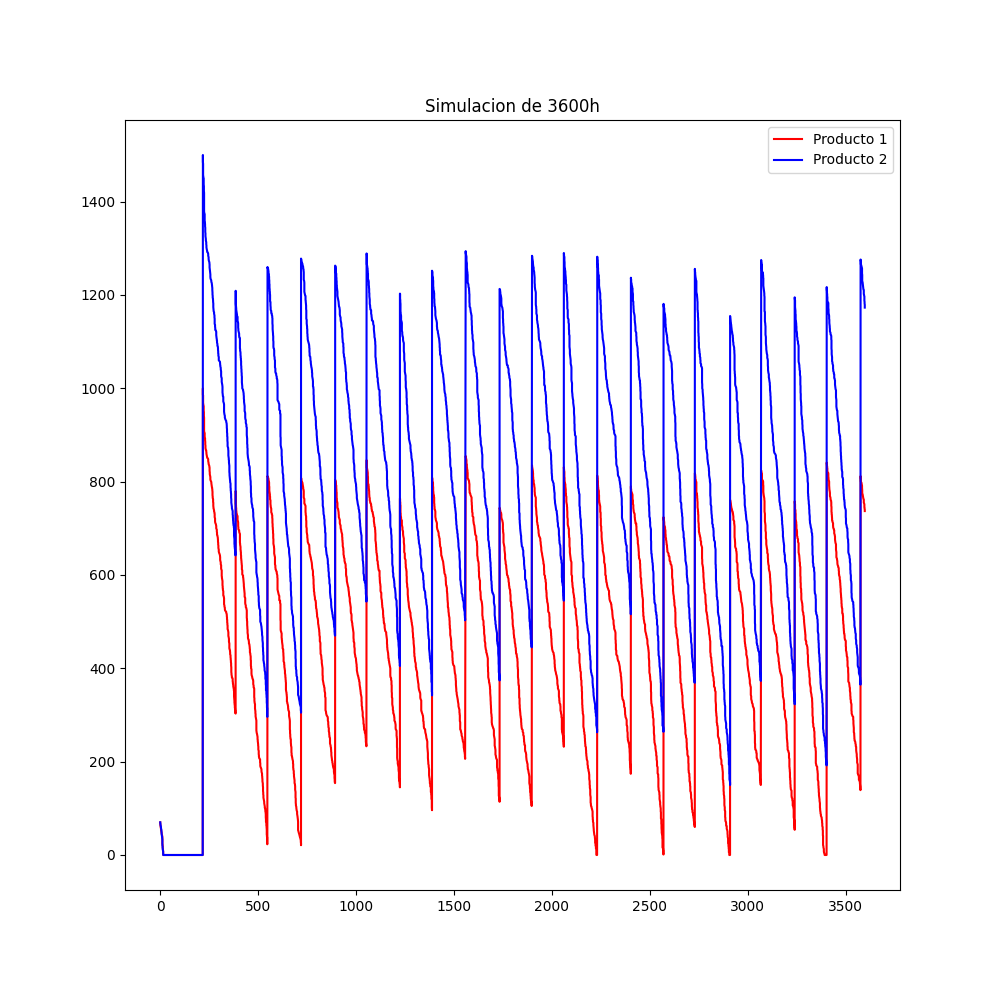
\includegraphics[width=0.9\textwidth]{include/sim.png}
		\caption{Estado del almacén de ambos productos durante la simulación}
	\end{figure}

\newpage
	
	\begin{figure}[H]
		\centering
		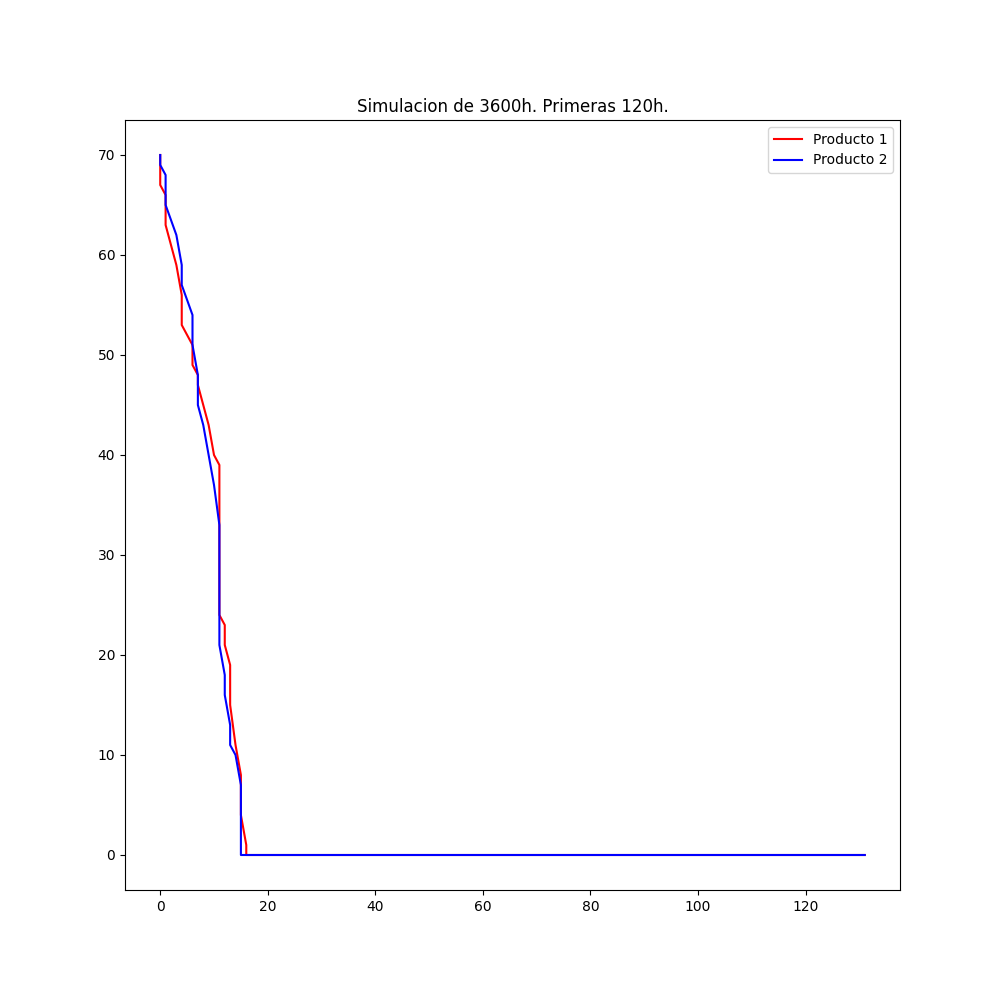
\includegraphics[width=0.9\textwidth]{include/sim_first5h.png}
		\caption{Estado del almacén de ambos productos durante las primeras 5 horas de simulación}
	\end{figure}
\newpage

	\subsection{Simulación del problema con metaheurísticas. Identificación de política de pedidos óptima.}
	
	\subsubsection{Implementación}
	El proceso de recocido simulado genera N iteraciones de la simulación, modificando algunos de los valores
	
	\subsubsection{Resultados}
	
\newpage
	\section*{Bibliografía}
	\addcontentsline{toc}{section}{Bibliografía}
	\bibliography{include/references}
	\bibliographystyle{IEEEtran}
	
\end{document}